\documentclass[conference]{IEEEtran}
\IEEEoverridecommandlockouts

\usepackage{cite}
\usepackage{amsmath,amssymb,amsfonts}
\usepackage{graphicx}
\usepackage{textcomp}
\usepackage{xcolor}
\usepackage{hyperref}
\usepackage{booktabs}
\usepackage{array}
\usepackage{float}
\hypersetup{
    colorlinks=true,
    linkcolor=blue,
    urlcolor=blue,
    citecolor=blue
}


\def\BibTeX{{\rm B\kern-.05em{\sc i\kern-.025em b}\kern-.08em
    T\kern-.1667em\lower.7ex\hbox{E}\kern-.125emX}}

\begin{document}

\title{Mini OS: A Freestanding Operating System Simulation\\
{\large Implementing Core OS Subsystems in C99 Without Standard Libraries}}

\author{
  \IEEEauthorblockN{Vaiditya Tanwar}
  \IEEEauthorblockA{
    \textit{Newton School of Technology}\\
    \textit{Rishihood University}\\
    Enrollment No.: 230086\\
    vaiditya.t23csai@nst.rishihood.edu.in
  }
}

\maketitle

% ─────────────────────────────────────────────────────────────────────
\begin{abstract}
Mini OS is a freestanding operating system simulation written entirely in C99, with no dependency on the C standard library for core logic. The project implements, from first principles, all major OS subsystems: a first-fit free-list heap allocator with forward coalescing, a custom string library using raw pointer arithmetic, an inode-based virtual filesystem, a preemptive task scheduler driven by \texttt{SIGALRM} timer interrupts, a shell script engine supporting foreground and background execution, and a double-buffered ANSI terminal renderer. The system runs as an interactive Unix process and provides a command-line shell as the primary user interface. Every design decision maps directly to a real operating system concept, making this project both a functional system and an educational model of OS internals. The implementation enforces strict module isolation, signal-safe interrupt handling, and unified memory management across all subsystems. Unit tests cover all core libraries. This paper describes the architecture, methodology, and design rationale of each subsystem, and identifies directions for future extension.
\end{abstract}

\begin{IEEEkeywords}
operating systems, memory management, virtual filesystem, preemptive scheduling, signal handling, systems programming, C99
\end{IEEEkeywords}

% ─────────────────────────────────────────────────────────────────────
\section{Introduction}

Modern operating systems are complex, layered systems that manage hardware resources and present abstractions to user programs. Understanding how these abstractions are implemented — heaps, filesystems, schedulers, device drivers — is fundamental to systems programming yet often opaque to students who interact with them only through library interfaces.

Mini OS addresses this gap by re-implementing each OS subsystem from scratch in C99, using a static memory array as ``physical RAM,'' POSIX signals as timer interrupts, \texttt{termios} for raw device I/O, and a 64-slot inode table as a disk partition. The result is a self-contained, interactive operating system simulation that demonstrates, in runnable code, how real OSes solve the problems of memory allocation, file organization, process scheduling, and secure I/O.

The project was built in two phases. Phase~1 (April 7--14) established the core subsystems: memory allocator, string library, screen and keyboard drivers, math engine, virtual filesystem, shell REPL, and cooperative task scheduler, with a full unit test suite. Phase~2 (April 22--24) upgraded the cooperative scheduler to a preemptive model using \texttt{SIGALRM} and added a shell script engine supporting both synchronous (foreground) and asynchronous (background) script execution.

\begin{figure}[H]
  \centering
  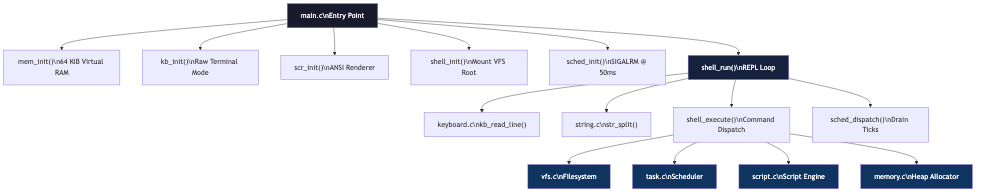
\includegraphics[width=\columnwidth]{figures/arch.png}
  \caption{System architecture and module dependency graph. All heap allocations across every subsystem flow through \texttt{memory.c}.}
  \label{fig:arch}
\end{figure}

% ─────────────────────────────────────────────────────────────────────
\section{Methodology}

\subsection{Memory Management}

The heap allocator (\texttt{memory.c}) implements a \textbf{first-fit free list} over a 64\,KiB static array declared in \texttt{main.c}:

\begin{verbatim}
static char virtual_ram[VIRTUAL_RAM_SIZE]; // 65536 bytes
mem_init(virtual_ram, VIRTUAL_RAM_SIZE);
\end{verbatim}

Each block is prefixed by a \texttt{BlockHeader} struct storing the total block size (including header), a free flag, and a next pointer forming a singly linked list:

\begin{verbatim}
typedef struct BlockHeader {
    size_t              size;
    int                 is_free;
    struct BlockHeader *next;
} BlockHeader;
\end{verbatim}

\textbf{Allocation} walks the list for the first free block satisfying the requested size. If the block remainder exceeds \texttt{MIN\_BLOCK\_SIZE}, it is split into an allocated block and a new free block, minimizing wasted space. All returned pointers are aligned to 8-byte boundaries via the \texttt{ALIGN} macro.

\textbf{Deallocation} includes three safety mechanisms: (1) a bounds check rejecting pointers outside the heap region, (2) a double-free guard that silently ignores attempts to free an already-free block, and (3) \textbf{forward coalescing} — after marking a block free, the entire list is scanned and all adjacent free blocks are merged. Coalescing prevents fragmentation from accumulating across many alloc/free cycles and is verified by the stress test in \texttt{test\_memory.c} (1{,}000 allocation/free cycles with full heap recovery).

\begin{figure}[H]
  \centering
  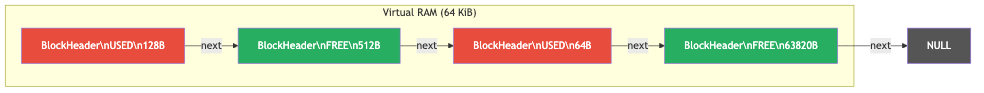
\includegraphics[width=\columnwidth]{figures/memory.png}
  \caption{Heap free list after several allocations. Red = USED, Green = FREE. Forward coalescing merges adjacent green blocks on every \texttt{mem\_free}.}
  \label{fig:memory}
\end{figure}

Every subsystem — VFS file data, task state structs, script line buffers — allocates exclusively through \texttt{mem\_alloc} and \texttt{mem\_free}. This unified allocation model allows \texttt{memmap} to produce a complete, accurate picture of system memory at any moment.

\subsection{File System}

The virtual filesystem (\texttt{vfs.c}) is modelled directly on Unix inode semantics. A 64-slot \texttt{inode\_table} stores all file and directory metadata; file content is heap-allocated via \texttt{mem\_alloc}.

\begin{verbatim}
typedef struct {
    char  name[MAX_NAME_LEN];
    int   size, is_dir, is_used;
    char *data;   /* heap pointer via memory.c */
    int   parent; /* parent inode index; -1 = root */
} Inode;
\end{verbatim}

A \texttt{Superblock} tracks total file and directory counts and the current working directory inode index. The directory tree is represented implicitly through the \texttt{parent} field: to list a directory, all inodes with a matching \texttt{parent} index are enumerated. This mirrors how real on-disk filesystems organize entries.

Supported operations include \texttt{touch}, \texttt{mkdir}, \texttt{write}, \texttt{read}/\texttt{cat}, \texttt{rm}, \texttt{ls}, and \texttt{cd} (including \texttt{..} and \texttt{/} traversal). The \texttt{rm} operation verifies that directories are empty before deletion and frees file data back to the heap allocator, preventing memory leaks. The \texttt{vfs\_read\_to\_buf()} function exposes raw file content for consumption by the script engine without going through the terminal output path.

\subsection{Process Management}

\subsubsection{Task State Machine}

Tasks are represented as entries in an 8-slot table. Each entry holds a function pointer (\texttt{tick\_fn}), a heap-allocated state pointer, and a \texttt{TaskState} enum:

\begin{center}
\begin{tabular}{ll}
\toprule
\textbf{State} & \textbf{Behaviour} \\
\midrule
\texttt{TASK\_READY}    & \texttt{tick\_fn} is called on every scheduler dispatch \\
\texttt{TASK\_SLEEPING} & \texttt{sleep\_ticks} decrements; transitions to READY at 0 \\
\texttt{TASK\_DONE}     & Slot is reaped (freed) automatically on next pass \\
\bottomrule
\end{tabular}
\end{center}

\subsubsection{Preemptive Scheduler}

Phase~2 upgraded the scheduler from a cooperative model (manual \texttt{task\_tick\_all()} calls) to a preemptive model using \texttt{SIGALRM}. The design maps directly to hardware timer interrupt handling in a real kernel:

\begin{figure}[H]
  \centering
  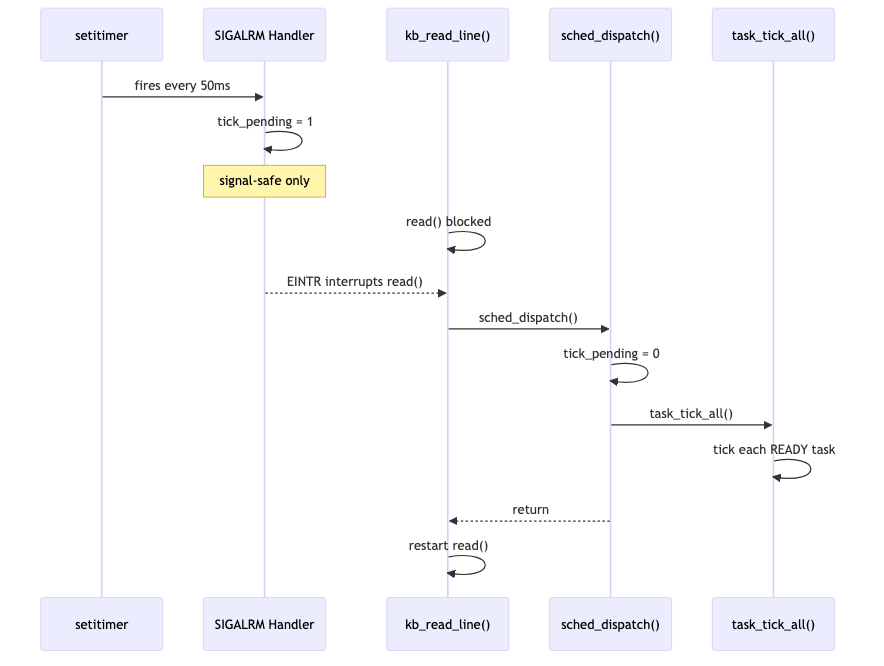
\includegraphics[width=\columnwidth]{figures/scheduler.png}
  \caption{Preemptive scheduler sequence. The signal handler (ISR) sets only a flag. \texttt{sched\_dispatch()} performs the real work in safe context.}
  \label{fig:scheduler}
\end{figure}

\texttt{sched\_init()} arms \texttt{setitimer(ITIMER\_REAL, 50\,ms)}. The signal handler sets a \texttt{volatile sig\_atomic\_t} flag and returns immediately — no \texttt{printf}, no \texttt{malloc}, no function calls. Signal-unsafe operations in a handler are undefined behaviour and can corrupt process state; the flag pattern is the POSIX-compliant solution. \texttt{sched\_dispatch()} clears the flag and calls \texttt{task\_tick\_all()} from normal execution context, mirroring how kernel schedulers run after saving the interrupted process's context.

\texttt{kb\_read\_line()} handles \texttt{EINTR} (the error returned when a blocking \texttt{read()} is interrupted by a signal) by calling \texttt{sched\_dispatch()} before restarting the read, ensuring background tasks tick continuously even during user input.

\subsubsection{Shell Script Engine}

Scripts are plain VFS files (one command per line; \texttt{\#} lines are comments). \texttt{script\_run\_fg()} executes lines synchronously by calling \texttt{shell\_execute()} for each — the same dispatch path as interactive commands. \texttt{script\_run\_bg()} allocates a \texttt{ScriptState} struct on the heap, loads the line table, and registers a \texttt{script\_bg\_tick} function as a scheduler task. Each 50\,ms tick executes one line; when all lines are consumed the task sets \texttt{TASK\_DONE} and the slot is reaped automatically.

\subsection{I/O Management}

\subsubsection{Keyboard Input}

\texttt{keyboard.c} uses \texttt{tcsetattr()} to configure the terminal in raw mode (\texttt{ICANON} and \texttt{ECHO} disabled, \texttt{VMIN=0}, \texttt{VTIME=0}). \texttt{kb\_read\_line()} switches to blocking mode for the read loop, handles backspace with cursor manipulation, filters control characters, decodes multi-byte arrow key escape sequences (\texttt{ESC[A/B/C/D}), and restarts on \texttt{EINTR}. The original terminal configuration is saved and restored via \texttt{atexit()}.

\subsubsection{Screen Output}

\texttt{screen.c} implements a double-buffered ANSI renderer with diff-based refresh. A logical \texttt{back} buffer accumulates all drawing calls; \texttt{scr\_refresh()} compares each cell against the physical \texttt{front} buffer and emits ANSI cursor-positioning and colour sequences only for changed cells. All output is accumulated in a local write buffer and flushed in a single \texttt{fputs()} call, eliminating flicker from multiple small writes. Console wrappers (\texttt{scr\_print}, \texttt{scr\_println}) are used throughout all modules for terminal output.

\subsection{Security, Error Handling, and Halt}

Mini OS treats correctness and safety as first-class concerns across all subsystems:

\textbf{Memory safety.} \texttt{mem\_free} performs bounds checking (pointer outside heap rejected), double-free protection (silently ignored), and NULL checking. \texttt{mem\_alloc} returns \texttt{NULL} on out-of-memory rather than crashing.

\textbf{Filesystem safety.} All VFS operations validate inputs: zero-length names are rejected, duplicate names in the same directory are rejected, directory removal is refused if the directory is non-empty, and writing to a directory path is refused with an explicit error.

\textbf{Signal safety.} The SIGALRM handler is strictly signal-safe: it performs no I/O, no allocation, and calls no non-reentrant functions. \texttt{SA\_RESTART} is set so interrupted restartable syscalls are handled by the kernel rather than requiring manual restarts.

\textbf{String safety.} \texttt{str\_copy} and \texttt{str\_concat} always bound-check against the supplied \texttt{max\_len} and always null-terminate. \texttt{str\_compare} handles NULL arguments explicitly. Numeric conversions (\texttt{str\_atoi}, \texttt{str\_itoa}) handle edge cases (zero, negatives, non-numeric input, INT\_MIN) without undefined behaviour.

\textbf{Halt.} The \texttt{exit} command sets \texttt{shell\_running = 0}, causes the REPL loop to terminate, and \texttt{kb\_restore()} is called before \texttt{main()} returns, restoring the terminal to its original state. The \texttt{atexit()} registration of \texttt{kb\_restore()} ensures restoration even on abnormal termination.

\textbf{Task safety.} \texttt{task\_kill} validates the task ID range and active flag before freeing state. Background script tasks that exhaust their line table self-transition to \texttt{TASK\_DONE} rather than requiring external cleanup.

% ─────────────────────────────────────────────────────────────────────
\section{Results and Evaluation}

\begin{table}[H]
\centering
\caption{Unit Test Results}
\begin{tabular}{llr}
\toprule
\textbf{Suite} & \textbf{Coverage} & \textbf{Tests} \\
\midrule
\texttt{test\_memory} & Alloc, free, split, coalesce, OOM, stress & 17 \\
\texttt{test\_math}   & Arithmetic, spatial, RNG determinism     & 18 \\
\texttt{test\_string} & All string functions incl. tokenizer     & 28 \\
\texttt{test\_shell}  & Integration: parse $\to$ execute pipeline  & 22 \\
\midrule
\textbf{Total}        &                                          & \textbf{85} \\
\bottomrule
\end{tabular}
\label{tab:tests}
\end{table}

All 85 tests pass. The memory stress test runs 1{,}000 allocation/free cycles across 10 iterations (100 allocations per cycle, variable sizes 32--96 bytes) and verifies that available memory is fully recovered and the heap coalesces to a single block after each cycle. The string tokenizer test exercises leading/trailing delimiters, multiple consecutive delimiters, empty input, and single-token strings. The shell integration test traces a full \texttt{echo hello world} command from tokenization through output reconstruction.

% ─────────────────────────────────────────────────────────────────────
\section{Future Scope}

\textbf{Syscall interface.} A formal \texttt{sys\_*} dispatch table (analogous to a system call table) would cleanly separate ``userspace'' shell commands from ``kernel'' subsystem operations, enforcing the privilege boundary that real OSes maintain.

\textbf{Inter-process communication.} Pipes (\texttt{cmd1 | cmd2}) and message queues between tasks would enable composable commands and demonstrate IPC primitives (shared memory, ring buffers, semaphores).

\textbf{Command history and tab completion.} Storing the last $N$ commands in a ring buffer and completing filenames by scanning VFS inodes would significantly improve shell usability with minimal complexity.

\textbf{File permissions and timestamps.} Adding \texttt{owner}, \texttt{mode}, and \texttt{created\_at} fields to inodes and surfacing them in \texttt{ls -l} output would complete the Unix inode model.

\textbf{Network simulation.} A loopback ``network'' with \texttt{send}/\texttt{recv} primitives and a virtual socket table would extend the I/O subsystem to cover the network layer.

\textbf{Bootloader simulation.} A \texttt{boot.c} stage that loads the OS image from a simulated sector array before \texttt{main()} would model the BIOS/UEFI handoff to the kernel.

% ─────────────────────────────────────────────────────────────────────
\begin{thebibliography}{00}

\bibitem{silberschatz}
A. Silberschatz, P. B. Galvin, and G. Gagne,
\textit{Operating System Concepts}, 10th ed.
Hoboken, NJ: Wiley, 2018.

\bibitem{tanenbaum}
A. S. Tanenbaum and H. Bos,
\textit{Modern Operating Systems}, 4th ed.
Upper Saddle River, NJ: Pearson, 2015.

\bibitem{knuth}
D. E. Knuth,
\textit{The Art of Computer Programming, Vol.\ 1: Fundamental Algorithms}, 3rd ed.
Reading, MA: Addison-Wesley, 1997.

\bibitem{stevens}
W. R. Stevens and S. A. Rago,
\textit{Advanced Programming in the UNIX Environment}, 3rd ed.
Upper Saddle River, NJ: Addison-Wesley, 2013.

\bibitem{posix}
IEEE and The Open Group,
\textit{The Open Group Base Specifications Issue 7 (POSIX.1-2017)},
IEEE Std 1003.1-2017. [Online].
Available: \url{https://pubs.opengroup.org/onlinepubs/9699919799/}

\bibitem{kernighan}
B. W. Kernighan and D. M. Ritchie,
\textit{The C Programming Language}, 2nd ed.
Englewood Cliffs, NJ: Prentice Hall, 1988.

\bibitem{bovet}
D. P. Bovet and M. Cesati,
\textit{Understanding the Linux Kernel}, 3rd ed.
Sebastopol, CA: O'Reilly Media, 2005.

\end{thebibliography}

\end{document}
